\documentclass[aps,prc,reprint,amsmath,nofootinbib]{revtex4-1}

\usepackage{hyperref}
\usepackage{graphicx}
\graphicspath{{fig/}}

\usepackage{tikz}
\usetikzlibrary{shapes,calc,matrix}

\usepackage{mdwlist}
\renewcommand\labelitemi{\raisebox{.3ex}{\tiny$\bullet$}}

\newcommand{\trento}{T\raisebox{-.5ex}{R}ENTo}
\newcommand{\nch}{N_\text{ch}}
\newcommand{\eccratio}{\sqrt{\langle \varepsilon_2^2 \rangle}/\sqrt{\langle \varepsilon_3^2 \rangle}^{\,0.6}}

\begin{document}

\title{An effective model for entropy deposition in high-energy pp, pA, and AA collisions}

\author{J.\ Scott Moreland}
\author{Jonah E.\ Bernhard}
\author{Steffen A.\ Bass}
\affiliation{Department of Physics, Duke University, Durham, NC 27708-0305}

\date{\today}


\begin{abstract}
  We introduce \trento, a new initial condition model for high-energy nuclear collisions based on eikonal entropy deposition via a ``reduced thickness'' function.
  The model simultaneously predicts the shapes of experimental proton-proton, proton-nucleus, and nucleus-nucleus multiplicity distributions, and generates nucleus-nucleus eccentricity harmonics consistent with experimental flow constraints.
  In addition, the model provides a possible resolution to the ``knee'' problem in ultra-central uranium-uranium collisions.
\end{abstract}


\maketitle

%\section{Introduction}

Over the last decade, the ultra-relativistic heavy-ion collision programs at the Relativistic Heavy Ion Collider (RHIC) and the Large Hadron Collider (LHC) have succeeded in producing and exploring a novel, highly excited phase of QCD matter dubbed the strongly-interacting Quark-Gluon Plasma (sQGP)
\cite{Arsene:2004fa,Adcox:2004mh,Back:2004je,Adams:2005dq,Gyulassy:2004zy,Muller:2006ee,Muller:2012zq}.
A major goal of current research is the quantification of fundamental sQGP properties, typically accomplished by matching experimental measurements to computational models for the full spacetime evolution of heavy-ion collisions \cite{Petersen:2010zt,Novak:2013bqa}.
While viscous relativistic fluid dynamics provides a stable, well-tested description of the thermalized sQGP medium \cite{Baier:2006gy,Song:2007ux,Luzum:2008cw,Schenke:2010rr,Shen:2011eg,Shen:2014vra}, the initial state of the collision lacks a standard description and is modeled by numerous approaches in both strong and weak coupling limits \cite{Schenke:2012wb,vanderSchee:2013pia,Berges:2014yta,Kurkela:2014tea}.

Initial condition models generate profiles of energy or entropy at the sQGP thermalization time which are then evolved by fluid dynamics.
The most widely-used prescription is the two-component Monte Carlo Glauber model, which determines participating nucleons via optical overlap and deposits energy or entropy for each participant and binary nucleon-nucleon collision.
Despite its simplicity, the Glauber model has qualitatively fit many experimental measurements \cite{Miller:2007ri}.

Recently, a new constituent-quark participant model described the transverse-energy distributions of proton-proton, deuteron-gold, and gold-gold collisions at RHIC without invoking binary collision scaling \cite{PhysRevC.89.044905}.
This may suggest that the two-component wounded nucleon and binary collision ansatz is merely a proxy for quark participant scaling in nucleus-nucleus collisions.

The state-of-the-art model is IP-Glasma \cite{Schenke:2012wb}.
It uses color-glass condensate (CGC) effective field theory \cite{McLerran:1993ni,McLerran:1993ka,Gelis:2010nm} and classical Yang-Mills evolution to create a \emph{dynamical} description of the pre-equilibrium stage of the collision---unlike the Glauber model and its relatives, which ignore pre-equilibrium dynamics and skip directly to sQGP thermalization.
IP-Glasma quantitatively describes the latest event-by-event data on higher order flow harmonics and a variety of other observables \cite{Schenke:2014zha}.
However, the explicit treatment of pre-sQGP time-evolution comes at a significant computational cost.

In this work we introduce \trento, a new initial condition model for high-energy proton-proton, proton-nucleus, and nucleus-nucleus collisions.
It is an \emph{effective} model, intended to generate realistic Monte Carlo initial entropy profiles without assuming specific physical mechanisms for entropy production, pre-equilibrium dynamics, or thermalization.

%\section{The Model}

Suppose a pair of projectiles labeled $A$, $B$ collide along beam axis $z$.  Each projectile is represented by
the beam-integrated density of its nuclear matter, typically called a nuclear thickness:
\begin{equation}
  T_{A,B}(x, y) = \int dz \, \rho_{A,B}(x, y, z).
\end{equation}
The construction of the thickness functions will be addressed shortly; first, we postulate the following:
\begin{enumerate}
  \item The eikonal approximation is valid:  entropy is produced if $T_A$ and $T_B$ eikonally overlap.
  \item There exists a scalar field $f(T_A, T_B)$ which converts projectile thicknesses into entropy
    deposition.
\end{enumerate}
The function $f$ is proportional to the entropy created at mid-rapidity and at the hydrodynamic thermalization
time:
\begin{equation}
  f \propto dS/dy \, |_{\tau = \tau_0}.
\end{equation}
It should provide an effective description of early collision dynamics:  it need not arise from a
first-principles calculation, but it must obey basic physical constraints.

With this in mind, we introduce for $f$ the \emph{reduced thickness}
\begin{equation}
  f = T_R(p; T_A, T_B) \equiv \biggl( \frac{T_A^p + T_B^p}{2} \biggr)^{1/p},
  \label{eq:tr}
\end{equation}
so named because it takes two thicknesses $T_A$, $T_B$ and ``reduces'' them to a third thickness, similar to a
reduced mass.  The dimensionless parameter $p$ may take any real value in $(-\infty, \infty)$ and is to be
determined by experiment.  This functional form---known as the generalized mean---simplifies to arithmetic,
geometric, and harmonic means for certain values of $p$, i.e.
\begin{equation}
  T_R(p; T_A, T_B) =
  \begin{cases}
    \dfrac{T_A + T_B}{2} & p = 1 \text{ (arithmetic)}, \\[2ex]
    \sqrt{T_A T_B} & p = 0 \text{ (geometric)}, \\[2ex]
    \dfrac{2\, T_A T_B}{T_A + T_B} & p = -1 \text{ (harmonic)}. \\
  \end{cases}
\end{equation}
More generally, $p$ quantifies the attenuation of entropy production in asymmetric ($T_A \neq T_B$) regions of
the collision, as demonstrated in FIG.~\ref{fig:saturation}.  As $p$ \emph{decreases}, the degree of
attenuation \emph{increases}.  This significantly impacts the behavior of the model, for instance $p=1$ is
precisely a participant nucleon model, while $-1 \lesssim p \lesssim 0$ mimics saturation in CGC-based models.

The reduced thickness possesses several other key properties.  It is
\begin{enumerate*}
  \renewcommand{\labelenumi}{(\alph{enumi})}
  \item continuous and monotonically increasing: \\
    if $T_A \leq T_A'$ and $T_B \leq T_B'$, then $T_R \leq T_R'$;
  \item symmetric in the projectile thicknesses: \\
    $T_R(p; T_A, T_B) = T_R(p; T_B, T_A)$;
  \item independent of $p$ when the thicknesses are equal: \\
    $T_R(p; T, T) = T$; and
  \item vanishes when $T_A$ and $T_B$ vanish: $T_R(p; 0, 0) = 0$. \\
    In fact, for $p \leq 0$, $T_R$ vanishes if \emph{either} $T_A$ or $T_B$ do.
    On the other hand, positive values of $p$ introduce small violations of the eikonal entropy production postulate, similar to a Glauber model.
\end{enumerate*}

Finally, the reduced thickness provides the basis of the model name:
\trento, for Thickness-Reduced Event-by-event Nuclear Topology.

\begin{figure}[t]
  \includegraphics{saturation}
  \caption{
    \label{fig:saturation}
    Attenuation of the reduced thickness.  Thickness $T_B$ is fixed to one (in arbitrary units) while $T_A$ is
    varied.  The corresponding $T_R$ are shown for $p = 1$, 0, $-1$ (green, blue, and red).
  }
\end{figure}

We now detail the construction of the thickness functions $T_{A,B}(x, y)$, which combined with the definition
of the reduced thickness completes the specification of the model.  The procedure is constructed from the
ground up to handle a variety of collision systems; we begin with the simplest case.

%\subsection{Proton-proton collisions}

Consider a collision of two protons $A$, $B$ with impact parameter $b$ along the $x$-direction and nuclear densities
\begin{equation}
  \rho_{A,B} = \rho_\text{proton}(x \pm b/2, y, z),
\end{equation}
and assume that the integral $\int dz \, \rho_\text{proton}$ either has a closed form or may be evaluated numerically, so that the proton thickness functions can be calculated.
The protons collide with probability \cite{dEnterria:2010hd}
\begin{equation}
  P_\text{coll} = 1 - \exp\biggl[ -\sigma_{gg} \int dx \, dy \int dz \, \rho_A \int dz \, \rho_B \biggr],
  \label{eq:pcoll}
\end{equation}
where the integral in the exponential is the overlap integral of the proton thickness functions and
$\sigma_{gg}$ is an effective parton-parton cross-section tuned so that the total proton-proton
cross-section equals the experimental inelastic nucleon-nucleon cross-section $\sigma_{NN}$.

$P_\text{coll}$ is sampled once to determine if the protons collide; assuming they do, each is assigned a \emph{fluctuated} thickness
\begin{equation}
  T_{A,B}(x, y) = \gamma_{A,B} \int dz \, \rho_{A,B}(x, y, z),
\end{equation}
where $\gamma_{A,B}$ are independent random numbers sampled from a gamma distribution with unit mean,
\begin{equation}
  P(\gamma; k) \propto \gamma^{k-1} e^{-\gamma/k},
  \label{eq:gamma}
\end{equation}
with the shape parameter $k > 0$ to be fixed by experiment.  The gamma distribution is chosen for its
flexibility---it is exponential for $k = 1$ and becomes Gaussian for large $k$---and because it is the
continuous analog of the negative binomial distribution, which has historically been used to fit proton-proton
multiplicity fluctuations.

With the projectile thickness functions in hand, the reduced thickness is calculated to furnish the initial transverse entropy profile up to an overall normalization factor,
\begin{equation}
dS/dy \, |_{\tau = \tau_0} \propto T_R(p; T_A, T_B).
\end{equation}

\begin{figure*}[t]
  \includegraphics{multdist}
  \caption{
    \label{fig:multdist}
    Multiplicity distributions for proton-proton, proton-lead, and lead-lead collisions.  The blue histograms
    are \protect\trento\ results from $10^6$ minimum-bias events for each collision system, all with reduced
    thickness parameter $p = 0$ (geometric mean) and gamma fluctuation parameter $k = 0.8$.  The normalization
    constants indicated in the legends are tuned to match the experimental distributions
    (points with error bars) from ALICE \cite{Aamodt:2010ft,Abelev:2014mda}.
  }
\end{figure*}

%\subsection{Larger systems p+A and A+A}

Composite collision systems such as proton-nucleus and nucleus-nucleus are essentially treated as
superpositions of proton-proton collisions.
A set of nucleon positions is chosen for each projectile $A$, $B$, typically by sampling an uncorrelated Woods-Saxon distribution or from more realistic correlated nuclear configurations when available \cite{Alvioli:2009ab}.
The collision probability \eqref{eq:pcoll} is sampled for each pairwise interaction and those nucleons that collide with at least one partner are labeled ``participants'' while the rest are discarded.
The fluctuated thickness function of nucleus $A$ then reads
\begin{equation}
  T_A = \sum_i \gamma_i \int dz \, \rho_\text{proton}(x - x_i, y - y_i, z - z_i),
  \label{eq:nuc-thickness}
\end{equation}
where $\gamma_i$ and $(x_i, y_i, z_i)$ are the random fluctuation factor and position, respectively, of participant $i$ in nucleus $A$.
$T_B$ follows analogously.

This completes the construction of \trento.
In summary, the model deposits entropy proportional to the reduced thickness function \eqref{eq:tr}.
The reduced thickness is defined as the generalized mean of fluctuated projectile thickness functions \eqref{eq:nuc-thickness}, where the projectile thicknesses consist of \emph{only} participant nucleons, each independently fluctuated by a gamma random number \eqref{eq:gamma}.

%\section{Model Applications}

We now demonstrate \trento's ability to simultaneously describe a wide range of collision systems.
Note that the reduced thickness parameter $p$, gamma fluctuation parameter $k$, and nucleon profile $\rho_\text{proton}$ are not rigorously constrained---to do so would require a systematic model-to-data comparison which is beyond the scope of this work.
Therefore, the following results do not necessarily represent the best-fit of the model to data.

\begin{figure*}[t]
  \includegraphics{eccentricity}
  \caption{
    \label{fig:eccen}
    Left and middle plots:  Eccentricity harmonics $\varepsilon_2$ and $\varepsilon_3$ as a function of centrality
    for reduced thickness parameters $p = 1$, 0, $-1$ (green, blue, and red).  Right plot:  Ratio of the rms eccentricities
    $\eccratio$ against the experimentally allowed region (grey band) from \cite{Retinskaya:2013gca}.  Note that the centrality
    axis has a different range in the ratio plot.
  }
\end{figure*}

%\subsection{Multiplicity distributions}

The experimentally observed charged-particle multiplicity $\nch$ is to a very good approximation proportional to the total initial entropy \cite{Song:2008si}, and hence proportional to the integrated reduced thickness:
\begin{equation}
  \nch \propto \int dx \, dy \, T_R.
\end{equation}
To compare with experiment, we generate a large ensemble of minimum-bias events, integrate their $T_R$ profiles, and rescale by an overall normalization constant.

The left panel of FIG.~\ref{fig:multdist} shows the $\nch$ distribution from $10^6$ proton-proton simulations
using reduced thickness parameter $p = 0$ (geometric mean), gamma fluctuation parameter $k = 0.8$, and
Gaussian beam-integrated proton density
\begin{equation}
  \int dz \, \rho_\text{proton} = \frac{1}{2\pi B} \exp\biggr( -\frac{x^2 + y^2}{2B} \biggr)
\end{equation}
with effective area $B = (0.6\;\text{fm})^2$.
Proton-lead and lead-lead distributions (middle and right panels) use identical model parameters, except for the overall normalization factor, whose $\sim$20\% variation across collision systems is consistent with differences in experimental beam energy and kinematic cuts (annotated in the figure).

The $\nch$ distributions compare favorably with the corresponding experimental measurements by ALICE \cite{Aamodt:2010ft,Abelev:2014mda}.
\trento\ simultaneously reproduces the shapes of all three distributions, similarly to how the constituent-quark participant model fits the transverse-energy distributions of several collision systems at RHIC \cite{Adler:2013aqf}.

%\subsection{Eccentricity harmonics}

Eccentricity harmonics $\varepsilon_n$ are calculated using the definition
\begin{equation}
  \varepsilon_n e^{i n\phi} = -\frac{\int dx \, dy\, r^n e^{i n \phi} \, T_R}{\int dx \, dy \, r^n \, T_R}.
\end{equation}
Figure~\ref{fig:eccen} shows ellipticity $\varepsilon_2$ and triangularity $\varepsilon_3$ for lead-lead collisions as a function of centrality for reduced thickness $p = 1$,~0,~$-1$.  There is a clear trend of increasing eccentricity
(particularly $\varepsilon_2$) with decreasing $p$.  This may be understood by the attenuation property of the
reduced thickness:  as $p$ decreases, asymmetric regions of the collision produce less entropy, which
accentuates the elliptical overlap shape in non-central collisions and enhances their eccentricity.

In addition, we perform the test proposed by \cite{Retinskaya:2013gca}, which uses flow data and hydrodynamic calculations to determine an experimentally allowed band for the ratio of root-mean-square eccentricities $\eccratio$ as a function of centrality.
Among available initial condition models only IP-Glasma consistently falls within the allowed region.
As shown in the right panel of FIG.~\ref{fig:eccen}, \trento\ yields excellent agreement with the allowed band for $p = 0$ (geometric mean).

%\subsection{Ultracentral U+U collisions}

\begin{figure}[b]
  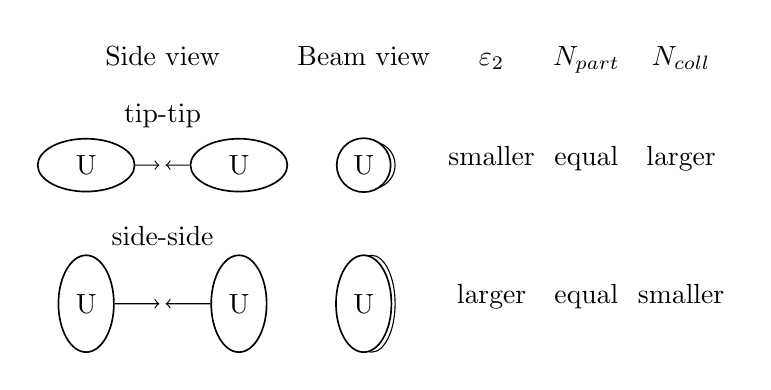
\begin{tikzpicture}[
    uranium/.style={draw, semithick, ellipse, anchor=center},
    small width/.style={minimum width=17},
    large width/.style={minimum width=35},
    small height/.style={minimum height=17},
    large height/.style={minimum height=35}
  ]
    \matrix (m) [matrix of nodes] {
      &[-5mm] Side view &[-5mm] & Beam view & $\varepsilon_2$ & $N_\text{part}$ & $N_\text{coll}$ \\[1ex]
      & tip-tip & & & & & \\
      |[uranium, large width, small height] (ttl)| U & &
      |[uranium, large width, small height] (ttr)| U &
      \node[draw, circle, small height, small width, xshift=1mm] {};
      \node[uranium, circle, small width, small height, fill=white] {U}; &
      smaller & equal & larger \\[2ex]
      & side-side & & & & & \\
      |[uranium, large height, small width] (ssl)| U & &
      |[uranium, large height, small width] (ssr)| U &
      \node[draw, ellipse, large height, small width, xshift=1mm] {};
      \node[uranium, large height, small width, fill=white] {U}; &
      larger & equal & smaller \\
    };
    \begin{scope}[->]
      \draw (ttl) -- ($(ttl)!.48!(ttr)$);
      \draw (ttr) -- ($(ttr)!.48!(ttl)$);
      \draw (ssl) -- ($(ssl)!.48!(ssr)$);
      \draw (ssr) -- ($(ssr)!.48!(ssl)$);
    \end{scope}
  \end{tikzpicture}
  \caption{
    \label{fig:uu-schematic}
    Comparison of tip-tip and side-side uranium-uranium collisions.
    Schematics are shown from a side view and looking down the beam axis, and the following quantities are compared:
    ellipticity $\varepsilon_2$, number of participating nucleons $N_\text{part}$, and number of binary nucleon-nucleon collisions $N_\text{coll}$.
  }
\end{figure}

\begin{figure}[b]
  \centering
  \includegraphics{uranium}
  \caption{
    \label{fig:uranium}
    Ellipticity $\varepsilon_2$ as a function of normalized charged-particle multiplicity
    $\nch/\langle\nch\rangle$ in ultra-central uranium-uranium and gold-gold collisions at RHIC.  The top and
    bottom plots show the top 0.1\% and 1\% (respectively) of collisions selected by number of spectators to
    mimic STAR's experimental ZDC selection \cite{FortheSTAR:2013bza}.  Blue points with error bars are binned
    \protect\trento\ results from $10^6$ events with reduced thickness parameter $p = 0$ (geometric mean) and
    gamma fluctuation parameter $k = 0.8$.  Blue lines are linear fits within
    $0.9~<~\nch/\langle\nch\rangle~<~1.1$.  Grey lines represent the analogous Glauber+NBD slopes calculated
    in \cite{FortheSTAR:2013bza}.
  }
\end{figure}

As a final novel application, we test the performance of \trento\ in ultra-central uranium-uranium collisions, where typical Glauber models are notably inconsistent with experimental data.
Unlike e.g.~gold and lead, uranium nuclei have a highly deformed prolate spheroidal shape, so uranium-uranium collisions may achieve maximal overlap via two distinct orientations:
``tip-tip'', in which the long axes of the spheroids are aligned with the beam axis and the overlap area is circular;
or ``side-side'', where the long axes are perpendicular to the beam axis and the overlap area is elliptical, as shown in FIG.~\ref{fig:uu-schematic}.
Hence side-side collisions will in general have larger initial-state ellipticity $\varepsilon_2$ and final-state elliptic flow $v_2$ than tip-tip.

In the two-component Glauber model, tip-tip collisions produce more binary nucleon-nucleon collisions than side-side, so tip-tip collisions have larger charged-particle multiplicity $\nch$.
Therefore, the most central uranium-uranium events are dominated by tip-tip collisions with maximal $\nch$ and small $v_2$, while side-side collisions have a smaller $\nch$ and somewhat larger $v_2$.
This predicted drop in elliptic flow as a function of $\nch$ is known as the ``knee'' \cite{Voloshin:2010ut}.

Recent data by STAR on uranium-uranium collisions exhibits no evidence of a knee \cite{FortheSTAR:2013bza,Wang:2014qxa}, at odds with Glauber model predictions.
It has been proposed that fluctuations could wash out the knee \cite{Rybczynski:2012av}, but a recent flow analysis suggests that it would still be visible \cite{osu}.

The reduced thickness ansatz \eqref{eq:tr} does not exhibit binary collision scaling and hence predicts a roughly constant ellipticity $\varepsilon_2$ in ultra-central uranium-uranium events, as shown in FIG.~\ref{fig:uranium}.
The slope of $\varepsilon_2$ as a function of $\nch$ is approximately equal for uranium-uranium and gold-gold, in contrast to the Glauber model which predicts a much steeper slope for uranium.
Short of conducting a full hydrodynamic analysis, \trento\ appears to be more consistent with STAR data than the Glauber model, and behaves similarly to IP-Glasma \cite{Wang:2014qxa}.

% \section{Summary}

In summary, we have developed \trento, a new model for the initial state of high-energy nuclear collisions based on eikonal deposition via a ``reduced thickness'' function.
The model simultaneously fits proton-proton, proton-nucleus, and nucleus-nucleus multiplicity distributions along with lead-lead eccentricity harmonics, and provides a possible resolution to the ``knee'' puzzle in ultra-central uranium-uranium collisions.

\trento\ is an effective model.
While it does not assume a particular physical mechanism for entropy production or include pre-equilibrium dynamics, it is computationally cheap, flexible by design, and mimics the characteristics of other initial condition models, e.g.~its multiplicity distributions are similar to constituent-quark participant model predictions, and eccentricity harmonics resemble those of IP-Glasma.

As a next step, we will couple the initial condition generator to viscous relativistic fluid dynamics as part of a complete simulation of the spacetime evolution of relativistic heavy-ion collisions \cite{Shen:2014vra}.
This will form the basis of a modern framework for extracting fundamental sQGP properties through systematic model-to-data comparison.

\medskip\noindent
\trento\ will be publicly released in early 2015 and made available at \url{github.com/Duke-QCD/trento}.
The community is encouraged to use, test, and contribute to the source code.

% \section*{Acknowledgements}

\medskip\noindent
We would like to thank Ulrich Heinz, Scott Pratt, Ron Soltz, and Berndt M\"uller for many helpful discussions and valuable feedback.
SAB is being supported by the U.S. Department of Energy Grant no.~DE-FG02-05ER41367,
JEB is supported through NSF grant no.~PHY-0941373,
and JSM acknowledges support by the DOE/NNSA Stockpile Stewardship Graduate Fellowship under grant no.~DE-FC52-08NA28752.

\bibliography{trento,duke-qcd-refs/Duke_QCD_refs}


\end{document}
